% !TeX spellcheck = it_IT
% !TEX encoding = utf8
% !TEX root = main.tex

\documentclass[parskip=half,
	fontsize=9pt,
	% chapterprefix=true,
	numbers=noenddot,
	bibliography=totoc]{scrbook}

\usepackage{etoolbox}
\makeatletter
\patchcmd{\scr@startchapter}{\if@openright\cleardoublepage\else\clearpage\fi}{}{}{}
\makeatother

\usepackage[utf8]{inputenc}
\usepackage[T1]{fontenc}
\usepackage[italian]{babel}
\usepackage{microtype}

\usepackage[square,numbers,sectionbib]{natbib}
\usepackage{chapterbib}

\PassOptionsToPackage{pdftex}{graphicx}
\usepackage{graphicx} 
\graphicspath{{Images/}{}}
\usepackage[outdir=./]{epstopdf}


% Golden ratio proportions on crown quarto with marginpar inside
\usepackage[includemp,
	paperwidth=18.90cm,
	paperheight=24.58cm,
	top=2.170cm,
	bottom=3.510cm,
	inner=2.1835cm,
	outer=2.1835cm,
	marginparwidth=4cm, % Fixed for now
	marginparsep=0.4cm]{geometry}

% For full bleed printing on crown quarto with 1/8 inch trim margin
% \usepackage[includemp,
%             paperwidth=19.54cm,
%             paperheight=25.22cm,
%             % showframe,
%             layoutwidth=18.90cm,
%             layoutheight=24.58cm,
%             layouthoffset=0.32cm,
%             layoutvoffset=0.32cm,
%             top=2.170cm,
%             bottom=3.510cm,
%             inner=2.1835cm,
%             outer=2.1835cm,
%             marginparwidth=4cm, % Fixed for now
%             marginparsep=0.4cm]{geometry}

% For printing on A4
% \usepackage[includemp,
%             a4paper,
%             layoutwidth=18.90cm,
%             layoutheight=24.58cm,
%             layouthoffset=1.05cm,
%             layoutvoffset=2.56cm,
%             top=2.170cm,
%             bottom=3.510cm,
%             inner=1.668cm,
%             outer=2.699cm,
%             marginparwidth=4cm, % Fixed for now
%             marginparsep=0.4cm]{geometry}


\usepackage{kpfonts}
\usepackage{amsmath,amssymb}        % AMS symbols and environments
\usepackage{mathtools}              % More math symbols and environments
\usepackage{amsthm}

\usepackage[hypcap=true,format=plain]{caption}   % Correctly placed anchors for hyperlinks
\usepackage{floatrow}               % Set up captions of floats
\usepackage{marginfix}              % Make marginpars float freely
\usepackage{metalogo}               % XeTeX logo
\usepackage{scrlayer-scrpage}       % Customise head and foot regions
%\usepackage[footnote]{snotez}       % Footnotes as sidenotes
\usepackage{marginnote}

\extrafloats{100}

% Figures and tables
\floatsetup[figure]{margins=hangoutside,
	facing=yes,
	capposition=beside,
	capbesideposition={center,outside},
	floatwidth=\textwidth}
\floatsetup[widefigure]{margins=hangoutside,
	facing=yes,
	capposition=bottom}
\floatsetup[table]{margins=hangoutside,
	facing=yes,
	capposition=beside,
	capbesideposition={center,outside},
	floatwidth=\textwidth}
\floatsetup[widetable]{margins=hangoutside,
	facing=yes,
	capposition=bottom}

% Sidenotes
%\setsidenotes{text-mark-format=\textsuperscript{\normalfont#1},
%	note-mark-format=#1:,
%	note-mark-sep=\enskip}

\renewpagestyle{scrheadings}{
	{\hspace{-\marginparwidth}\hspace{-\marginparsep}\makebox[\overflowingheadlen][l]{\makebox[2em][r]{\thepage}\quad\rule{1pt}{100pt}\quad{}\leftmark}}%
	{\makebox[\overflowingheadlen][r]{\rightmark\quad\rule{1pt}{100pt}\quad\makebox[2em][l]{\thepage}}}%
	{}
}{
{}%
{}%
{}
}
\renewpagestyle{plain.scrheadings}{
	{}%
	{}%
	{}
}{
{\thepage}%
{\makebox[\overflowingheadlen][r]{\thepage}}%
{}
}

%\cleardoublepage%
%\renewpagestyle{scrheadings}{
%	{\makebox[2em][r]{\thepage}\quad\rule{1pt}{100pt}\quad\leftmark}%
%	{\hfill\rightmark\quad\rule{1pt}{100pt}\quad\makebox[2em][l]{\thepage}}%
%	{}
%}{
%{}%
%{}%
%{}
%}
%\renewpagestyle{plain.scrheadings}{
%	{}%
%	{}%
%	{}
%}{
%{\thepage}%
%{\hfill\thepage}%
%{}
%}


\newlength{\overflowingheadlen}
\setlength{\overflowingheadlen}{\linewidth}
\addtolength{\overflowingheadlen}{\marginparsep}
\addtolength{\overflowingheadlen}{\marginparwidth}

\usepackage{lipsum}



\theoremstyle{definition}
\newtheorem{defn}{Definition}[section]
\theoremstyle{plain}
\newtheorem{thm}{Theorem}[section]
\newtheorem{prop}{Proposition}[section]
\newtheorem{cor}{Corollary}[section]
\newtheorem{lmm}{Lemma}[section]
\theoremstyle{remark}
\newtheorem*{recall}{Recall}
\newtheorem*{example}{Example}
\newtheorem*{remark}{Remark}

\usepackage{hyperref}
\title{Mathone - Versione originale}
\author{Erik Pillon}
\date{\today}
% ----------------------- BODY ------------------------
\begin{document}
\maketitle
\tableofcontents
\chapter*{Premessa}

Se trovate qualche equazione che vi sembra troppo difficile o che non capite, fate come fanno i matematici: dateci un'occhiata, cercate di coglierne il massimo possibile e saltatela semplicemente provando magari dopo qualche riga a ritornarci sopra e a ridarci una letta. La maggior parte delle volte una rotella scatterà nella vostra testa! 

% Penrose quotation
In un certo numero di luoghi in questo libro ho fatto ricorso a fornmle matematiche, senza !asciarmi spaventare dagli awerti­menti che vengono dati di solito: che ogni formula ridurrà del 50 per cento il numero dei lettori generici. Se tu sei uno dei lettori che si spaventano (come del resto accade ai più) davanti a qualsiasi formula matematica, ti raccomando un modo di procedere che normalmente adotto io stesso quando mi si presenta una riga così fastidiosa. Il procedimento consiste, più o meno, nell'ignorarla del tutto e passare semplicemente alla prossima riga di testo! Beh, non proprio così; si dovrebbe concedere alla formula se non un'attenta lettura almeno una scorsa generale, e poi passare oltre. 
Dopo un po', se ci si trova armati di nuova fiducia, si potrà tornare alla formula trascurata e cercare di coglierne qualche elemento saliente. Il testo stesso può essere utile per capire che cosa sia importante e che cosa si possa invece ignorare senza danno. Se così non è, non si abbia paura a ignorare una formula e passare
tranquillamente oltre. \cite{book:Penrose_imperatore}



% !TeX spellcheck = it_IT
% !TEX encoding = utf8
% !TEX root = main.tex

\chapter{Gauss - Il principe dei Matematici}
\begin{minipage}{1.46\linewidth}
	\begin{flushright}
		\emph{La matematica è la regina delle scienze \\ e la teoria dei numeri è la regina della matematica.}\\
		\vspace{0.5cm}
		\bfseries{Carl Friedrich Gauss} \\
		\textnormal{(Braunschweig, mercoledì 30 aprile 1777-\\Gottinga, Venerdì 23 febbraio 1855)}.
	\end{flushright}
\end{minipage}

Carl Friedrich Gauss è stato probabilmente il più poliedrico scienziato di tutti i tempi ed è stato il penultimo uomo a "sapere tutto" (è stato superato solo parecchio tempo dopo da un certo Poincaré). Durante la sua lunghissima e vastissima produzione scientifica, è stato matematico, fisico e astronomo.

Ha dato contributi fondamentali in tutte le branche della matematica e della fisica allora conosciute: dall'analisi matematica (sia reale che complessa vedi articolo sui numeri complessi) alla teoria dei numeri, statistica, calcolo numerico, geometria differenziale, geodesia, geofisica, al magnetismo e elettrostatica fino all'astronomia e all'ottica.

\marginpar{
	\captionsetup{type=figure}
	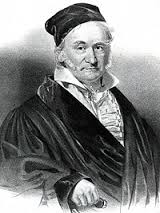
\includegraphics[width=\marginparwidth]{gauss.jpeg}
	\caption[Ritratto di Gauss]{Ritratto di Gauss}
	\label{fig:gauss}
}


Viene ricordato come Universalista, dal momento che eccelse in tutti i campi della disciplina nota ai suoi giorni.

\section{L'enfant prodige}

La storiografia insegna che fin dai primi anni di vita è stato considerato come un bambino prodigio. Molti aneddoti sono raccontati sulla sua infanzia, certi più famosi di altri, certi più accreditati di altri.

In particolare due sono particolarmente conosciuti:
\begin{itemize}
	\item Si narra che all'età di tre anni abbia corretto dei calcoli nelle finanze del padre; già dopo pochi mesi di vita, Gauss era in grado di fare operazioni algebriche, leggere e addirittura scrivere qualcosa.
	\item Un altro aneddoto racconta di come il suo il suo pigro insegnante, J.G. B\"{u}ttner, per tenere occupati i suoi allievi, ordinò loro di fare la somma dei numeri da 1 a 100. A quel tempo il giovane Gauss aveva solo 9 anni ma ugualmente dopo pochi minuti riuscì a consegnare la somma corretta: 5050.
\end{itemize}
Molte ipotesi sono state avanzate su quale metodo Gauss abbia usato: l'ipotesi più accreditata è che Carl si sia accorto che i numeri che differiscono della stessa distanza dagli estremi della serie danno sempre la stessa somma. Probabilmente mise in una riga i numeri da 1 a 100 e in una riga sotto i numeri da 100 a 1, e vide che ogni colonna dava come somma 101:

\[\begin{tabular}{cccccc}
$1$  &  $2$  &  $\dots $ & $99$  &  $100$ & $ + $\\
$100$  &  $99$  &  $\dots $ & $2$  &  $1$ & $ = $ \\ \hline
$101$  &  $101$  &  $\dots $ & $101$  &  $101$ & $  $\\
\end{tabular}\]

non restava dunque che fare il semplice calcolo $ \frac{100 \times 101}{2} $, ottenendo il risultato 5050 appunto. Aveva appena scoperto a 9 anni il risultato di quello che adesso noi chiameremo \emph{somma aritmetica}, o in simboli

\[\sum_{n=1}^{N} n  = \frac{N\times(N+1)}{2}  \] 

B\"uttner deve arrendersi davanti all'evidenza e dopo poco tempo supplicherà il il Duca di Brunswick di finanziare il giovane prodigio per potergli permettere di proseguire gli studi all'Università di Braunschweig prima (la più antica di Germania) e di Gottinga poi, dove trascorse gran parte del resto della sua esistenza.

\section{L'annus aureus}

Giunto all'Università Gauss ottenne una serie di notevoli risultati. Finalmente il suo genio poteva esprimersi al meglio e soprattutto poteva essere supportato e indirizzato da professori del suo livello, perlomeno fintanto che non vennero surclassati. In particolare il 1796 viene ricordato come l'anno d'oro. 
\marginpar{
	\captionsetup{type=figure}
	
\includegraphics[width=\marginparwidth]{firmaGauss}
	\caption{Firma di Gauss; si può notare come sia riuscito a conciliare nel suo nome il simbolo di integrale, la lettera greca $ \pi $ e il numero di Nepero $ e $}
	\label{fig:firmaGauss}
}
Tra le maggiori scoperte possiamo citare:
\begin{itemize}
	\item riuscì a dimostrare che un poligono regolare con un numero di lati che è un primo di Fermat è costruibile con riga e compasso. Questa fu una grande scoperta in un importante campo della matematica; la costruzione dei poligoni aveva occupato i matematici fin dall'epoca degli antichi greci, e la scoperta dette modo a Gauss di scegliere di intraprendere la carriera di matematico anziché di filologo.
	\item riuscì a costruire un eptadecagono;
	\item inventò l'aritmetica modulare, importantissimo strumento della teoria dei numeri che, solo per inciso, è la teoria dei numeri che tiene al sicuro i vostri e i miei soldi in banca;
	\item congetturò per primo la validità del teorema dei numeri primi, dando un'idea chiara di come i numeri primi siano distribuiti fra gli interi, cioè che se ne trovano sempre più di rado mano a mano che ci spostiamo verso l'infinito in un'ipotetica linea dei numeri, ma la loro distribuzione segue un andamento logaritmico;
	\item scoprì che tutti i numeri naturali sono rappresentabili al più come somma di tre numeri triangolari (Un numero intero positivo si dice triangolare se è uguale alla somma di una sequenza di numeri naturali consecutivi a partire da 1).
\end{itemize}

Aveva appena 19 anni. Per darvi l'idea, un ragazzo normale che studia matematica come il sottoscritto, non ha i mezzi per comprendere nemmeno un risultato. E pensatevi che molti dei suoi risultati sono stati pubblicati postumi o comunque dopo molti anni: voleva che fossero perfetti e riteneva molte delle dimostrazioni "non eleganti ".

A 22 anni completa il dottorato a Gottinga: nella sua tesi di dottorato viene riportata una nuova dimostrazione del teorema per il quale ogni funzione algebrica integrale di una variabile può essere risolta in fattori di primo o secondo grado. Aveva appena dimostrato il teorema fondamentale dell'algebra. Era entrato nella storia.

Sfortunatamente per lui, era troppo avanti rispetto ai suoi contemporanei; la sua commissione giudicatrice non aveva i mezzi necessari per capire la sua dimostrazione e verrà completamente appresa grazie al lavoro del geometra (in senso matematico, sia chiaro  ) francese Jordan e alla completa definizione dei numeri complessi.

Per non farsi mancare nulla, prima della sua morte pubblicò altre 4 dimostrazioni di questo teorema.

\section{La maturità}

Nel 1801, all'età di 24 anni, presenta il suo lavoro "\emph{Disquisitiones Arithmeticae}" che si rileva subito
come un dei contributi più importanti alla teoria dei numeri e una pietra miliare nel campo della matematica, al pari dei "\emph{Principia Mathematica}" di Newton.

In questo lavoro Gauss introduce ancora alcune nozioni basilari: i già citati numeri complessi, o immaginari- anche se di immaginario hanno poco- e la teoria delle congruenze. Il testo contiene anche una dimostrazione della legge di reciprocità quadratica (riguarda la risolubilità relativa in aritmetica modulare di due equazioni quadratiche correlate, dando le condizioni per cui entrambe, nessuna o una sola di esse hanno soluzione); un risultato che Gauss giudicava così importante che ne diede varie dimostrazioni durante la sua vita.

\subsection{Astronomia}
Per non farsi mancare nulla, si appassionò di li a poco tempo di astronomia: attraverso l'elaborazione di un nuovo metodo per la definizione delle orbite dei corpi celesti, infatti, riesce a calcolare la posizione dell'asteroide Cerere.

Il problema era stato lanciato da un astronomo italiano che dopo essere riuscito a tracciare la posizione dell'asteroide per un paio di mesi, ne aveva perso le tracce a causa del bagliore del sole. Dopo tre mesi di duro lavoro predisse la posizione di Cerere nel dicembre 1801 - appena un anno dopo il suo primo avvistamento - con un errore di appena mezzo grado.

Introdusse la costante gravitazionale di Gauss, e sviluppò il cosiddetto metodo dei minimi quadrati, una procedura usatissima ancora oggi per minimizzare l'impatto degli errori di misurazione. Questo risultato gli vale una posizione all'Osservatorio di Goettingen, di cui nel tempo ne diventerà direttore. Lo rimarrà fino alla morte.

\subsection{Probabilità}

Parallelamente ai lavori sull'astronomia, sviluppò una serie di fondamentali strumenti sull'analisi di dati e sulla distribuzione asintotica degli errori di misurazione. Stiamo parlando del teorema fondante della statistica e dell'econometria: il Teorema di Gauss-Markov.

\subsection{Geodetiche e Geometrie non euclidee}

Incaricato dal duca di Hannover nel 1821 a effettuare degli studi sui suoi possedimenti, Gauss diventa il principale studioso della cosiddetta geometria non-euclidea (purtroppo non mi posso dilungare troppo su questo punto, altrimenti un articolo non basterebbe per sviluppare solo questo paragrafo). Durante questo periodo sviluppa la teoria delle superfici e scopre il \emph{Teorema Egregium}(con tutto il rispetto per gli altri teoremi).

Parallelamente sviluppa anche quella che poi sarebbe stata chiamata "geometria sferica" negando il $ V $ postulato della geometria di Euclide. L'argomento però era scottante e Gauss decise di non pubblicare il risultato. Svariati anni dopo, il figlio di un suo intimo amico, dicasi Janos Bolyai, gli invia un lavoro rivoluzionario nel quale si sviluppano delle considerazioni sulla negazione del $ V $ postulato.

Gauss gli rivela privatamente che lo aveva anticipato di 30 anni. Questo amareggiò molto Janos, che mise fine ai rapporti con Gauss pensando che egli stesse rubando l'idea. Oggi la precedenza di Gauss è appurata ma quest'ultimo si rifiutò di pubblicare il lavoro per il timore della controversia.

\subsection{Elettromagnetismo}

Intorno al 1830, invece, si interessa di fisica e in particolare dei fenomeni che regolano l'elettromagnetismo. Inizia la collaborazione con il fisico Weber. Trova quella che sarà poi definita "legge di Gauss" o "Teorema del flusso" ossia la regola che sta alla base del comportamento delle particelle cariche statiche svelando il segreto che sta alla base della loro interazione: la distanza, in particolare il reciproco della distanza al quadrato.

La legge scopre insomma che tra due cariche elettriche ferme agisce una forza che dipende dalle cariche e dalla distanza a cui si trovano.

\subsection{Curiosità}

Curioso segnalare che il matematico ebbe l'idea di applicare il suo ingegno anche all'economia, questa volta non per soli e nobili fini scientifici ma anche per giustificati fini...personali. Infatti, si dedicò anche ad uno studio accurato dei mercati finanziari fino a guadagnare una fortuna personale considerevole.
\section{Morte e eredità}

Muore a Gottinga il 23 febbraio del 1855. Il suo genio era ormai leggenda.

\smallskip

Molte persone lo consideravano schivo e riservato. Ebbe due mogli ed entrambe morirono giovani. Ebbe 6 figli ed ebbe un rapporto travagliato con quasi tutti. Di tutti i figli di Gauss, si diceva che fosse Wilhelmina ad aver ereditato tratti del talento del padre, ma sfortunatamente morì giovane.

Sebbene avesse avuto alcuni studenti, Gauss era noto per detestare l'insegnamento, e prese parte ad un'unica conferenza scientifica, a Berlino nel 1828. Rare erano le collaborazioni con altri matematici, che lo consideravano solitario e austero. Tuttavia molti dei suoi studenti divennero importanti matematici:
\begin{itemize}
	\item Richard Dedekind, che diede fondamentali contributi alla logica e alla teoria dei numeri;
	\item Bernhard Riemann, che sviluppò sulle orme del maestro gli studi sulle geometrie non euclidee e sulle metriche di cui Einstein non poté fare a meno per la sua teoria della gravitazione;
	\item Friedrich Bessel, matematico, geometra e astronomo.
\end{itemize}
Prima che morisse, Sophie Germain (la seconda più grande matematica di tutti i tempi dopo Emmy Noether) fu raccomandata da Gauss affinché ricevesse anche lei la laurea honoris causa.

\bigskip

Questo è il mio primo articolo; se ti è piaciuto, se non ti è piaciuto per niente, se hai qualche annotazione, se mi sono dimenticato qualcosa che pensi sia rilevante (come se ce ne fossero poche :) ) o anche se solo vuoi confrontarti su qualche argomento che ho citato, ti prego di dirmelo; ogni commento è ben accetto ;)

Ho voluto iniziare la mia lista di articoli proprio con Gauss perché ritengo che sia stato il più grande di tutti i tempi e da quando ho iniziato a studiare, non ho ancora trovato una materia in cui prima o poi non si faccia uso di uno dei teoremi di Gauss. Era in anticipo sui suoi contemporanei di 30 o addirittura 50 anni. Senza di lui, probabilmente molti problemi avrebbero ancora il punto interrogativo al posto della soluzione.

\bibliography{bibliography}
\bibliographystyle{plain}


%\bibliography{bibliography}
%\bibliographystyle{plain}

% !TeX spellcheck = it_IT
% !TEX encoding = utf8

\chapter{Galois - Il Genio che non aveva tempo}
\begin{minipage}{1.46\linewidth}
		\begin{flushright}
			\emph{Sfortunatamente non si comprende come i libri scientifici più validi\\ siano quelli in cui l’autore indica chiaramente cosa non sa;\\ un autore fa infatti maggiormente del male ai suoi lettori\\ quando nasconde le difficoltà.}\\
			\vspace{0.5cm}
			\bfseries{Évariste Galois} \\
			\textnormal{(25 Ottobre 1811 – 31 Maggio 1832)}.
		\end{flushright}
\end{minipage}
\section{Évariste Galois - Il profeta}

Rivoluzionario, guerrafondaio, irrispettoso, insofferente verso la mediocrità, passionale e romantico. Del tutto incostante negli studi; geniale, ma refrattario all’istruzione formale e insofferente verso chi non era in grado di seguirlo mentre svolgeva complicati calcoli a mente (inclusi i propri esaminatori). Ancora diciannovenne aveva già risolto un problema che resisteva da secoli agli attacchi dei matematici, ma poiché pochissimi lo avevano capito, era convinto che sarebbe stato dimenticato.

\marginpar{ 
	\captionsetup{type=figure}
	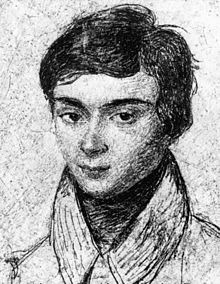
\includegraphics[width=\marginparwidth]{galois}
	\caption[Galois]{Una delle poche immagini di Galois pervenuteci}
	\label{fig:galois}
	}

Eppure la storia oggi gli rende giustizia ricordandolo come uno dei grandi della matematica. Forse il migliore algebrista di sempre. Ma chi era dunque Galois? Perché viene ricordato come l’ultimo matematico romantico?

\section{Una vita appassionata}

1811. L’Impero di Napoleone è all’apogeo. La campagna di Russia è alle porte. Ed è in questo clima che alle porte di Parigi, a Bourg-la-Reine, il 25 ottobre nasce Évariste Galois. Già da giovanissimo mostrò tutti i caratteri dell’énfant prodige. Leggeva e studiava manoscritti dei grandissimi del tempo: Lagrange, Gauss e Abel. Tuttavia mentre i suoi maestri di Matematica lo incoraggiavano e lo seguivano, quelli di tutte le altre materie lo ritenevano tutt’altro che un genio: non si applicava, non eccelleva in nessuna materia che non fosse la matematica e come se ciò non bastasse non si faceva nemmeno problemi a nascondere la sua insofferenza verso le cariche istituzionali che non gli andavano a genio.

Dal padre, sostenitore della Repubblica e sindaco del proprio villaggio nel periodo della Restaurazione, e dallo zio paterno (ufficiale napoleonico) prende la passione politica e comincia ad accostarsi al movimento repubblicano. Tuttavia il suicidio del padre assurdamente provocato per ragioni politiche segnerà profondamente lo spirito del giovane figlio.
\section{Un matematico incompreso}

Galois trascorreva talmente tanto tempo in profondi studi astratti che i suoi contemporanei non lo capivano. Eccone un esempio. Siamo nel 1829. Gaois ha 18 anni. I suoi lavori riguardavano le frazioni continue e la scoperta di nuovi insiemi numerici. Vuole entrare nel più prestigioso istituto di matematica dell’epoca: l’Accademia delle Scienze di Parigi. Presenta come domanda per l’ammissione alcune note sulla risoluzione tramite radicali di equazioni algebriche. Teniamo a mente che gran parte dell’algebra moderna viene da quelle note (se vuoi vedere qualche applicazione delle sue scoperte ecco un nostro recente articolo: I problemi con riga e compasso). I professori del tempo, restii alle idee di un diciottenne e abituati a ben altri calcoli, rifiutano il lavoro. Altri addirittura cestinano le note. Figuratevi come non reagì Galois che non solo si riteneva superiore alla sua commissione giudicatrice ma si mise addirittura a discutere con loro rinfacciandogli di non aver capito la portata delle sue idee.

Dovette a malincuore ripiegare sulla ben meno prestigiosa Scuola Normale.
\section{Il matematico romantico}

Cambiando scuola però i problemi non finirono. Durante i moti del 1830 ha i primi contrasti con le autorità. Ma non si piega. Al contrario, aumenta la propria posizione radicale. Viene prima arrestato, sbattuto in prigione e poi espulso dalla Scuola.

Alexandre Dumas a proposito dell’evento incriminato dell’arresto del giovane scrive:

All’improvviso, nel bel mezzo di una conversazione privata tra me e la persona seduta a sinistra, le mie orecchie sentirono il nome di Luigi Filippo, seguito da cinque o sei fischi. Mi voltai. A quindici o venti posti di distanza da me si stava svolgendo una delle scene più animate della serata. Un giovane che teneva nella stessa mano un bicchiere e un pugnale aperto cercava di farsi sentire dagli altri.
Si trattava di Évariste Galois. Riuscii a percepire solo che si trattava di una minaccia, e che era stato pronunciato il nome di Luigi Filippo. Il coltello aperto lasciava trasparire le intenzioni del giovane.

\section{Uno spirito passionale}

Rilasciato dal carcere nel 1832, si invaghisce di una ragazza. Da qui in poi ci sono ancora molte ombre sulle sua vita ma vi posso raccontare quella che la versione più accreditata racconta.

Lei si chiamava Stephanie Potterin du Motel e Galois l’aveva conosciuta solo pochi mesi prima. La relazione tra i due, però, si era interrotta quasi subito per ragioni che non sono note. Si sa solo che di lì a poco Galois fu sfidato a duello per difendere l’onere della donzella e a sfidarlo fu Ernest Duchatelet, “patriota” e una delle migliori pistole di Francia. E tirarsi indietro non era contemplabile all’epoca.

Oggi possiamo dire con un certo grado di sicurezza che quella di Galois fu probabilmente una congiura: tutto fu organizzato in modo che il giovine si trovasse nel posto giusto al momento sbagliato.

Galois sapeva che quella sarebbe stata la sua ultima notte. Rabbiosamente si rinchiude in casa per raccogliere tutti i suoi lavori e cercare di commentarli in modo che qualcuno possa un giorno riprenderli e fare in modo che le sue idee non vadano perdute. A margine dei fogli si può spesso leggere “non ho tempo… non ho tempo” proprio ad indicare l’ineluttabilità del momento e la pressione che si sentiva addosso… Provate ad immaginare cosa vuol dire avere la completa padronanza di un argomento che attanaglia la mente di matematici illustri da secoli, sapere che da lì a qualche ora la vostra morte si sta avvicinando e non avere il tempo per poter ordinare le vostre idee per evitare che vadano perdute!

Ed è proprio in questa notte che scrive la celebra lettera all’amico Chevalier. Essa è oggi considerata il suo testamento spirituale ai posteri, nonché base della moderna matematica. Nella stessa lettera si pregava Chavalier di far recapitare a Gauss e Jacobi tutti i lavori sulla sua opera di matematico.

“Pregherai pubblicamente Jacobi o Gauss di dare il loro parere, non sulla verità, ma sull’importanza dei teoremi. Dopo questo ci sarà, spero, qualcuno che troverà il suo profitto a decifrare tutto questo guazzabuglio”.

Personalmente, l’ultima volta che ho controllato il profitto si è trovato eccome!

Galois inoltre lascia nella lettera i principali teoremi della futura teoria dei gruppi che porta il suo nome e il legame profondo con la teoria della risoluzione algebrica delle equazioni.

\section{La teoria di Galois}

Prima di concludere però vorrei fare un breve accenno sulla teoria dei gruppi citando un esempio che ho trovato online a questa pagina.\footnote{Matematicamente un \emph{gruppo} è un insieme $ G $ munito di una operazione binaria $ \star $ che ad ogni coppia di elementi $ a,b $ di $ G $ associa un elemento, che indichiamo con $ a \star b $, appartenente a $ G $, rispettando i seguenti assiomi:
	\begin{itemize}
		\item \textbf{proprietà associativa}: dati $ a, b, c\in G $, vale $ (a\star b)\star c = a\star(b\star c) $.
		\item \textbf{esistenza dell'elemento neutro}: esiste in $ G $ un elemento \emph{neutro} $ e $  rispetto all'operazione $ \star $, cioè tale che $ a\star e = e\star a = a $ per ogni $ a\in G $.
		\item \textbf{esistenza dell'inverso}: ad ogni elemento $ a\in G $ è associato un elemento $ a' $, detto inverso di $ a $, tale che $ a\star a'=a'\star a=e $. 
	\end{itemize}
}

Considerate una gara di ciclismo a cui partecipano solo tre corridori. Quanti sono i possibili esiti della gara se i partecipanti non possono tagliare il traguardo contemporaneamente? Se indichiamo i ciclisti con i simboli $ A, B, C $, il problema dei possibili esiti della gara sta allora nel capire in quanti e quali modi si possono mettere in ordine gli oggetti $ A, B, C $.

Un modo efficace di procedere è di mettere in prima posizione, a turno, uno degli elementi e vedere cosa succede dopo, nelle altre posizioni. Per esempio, se il ciclista $ A $ finisce primo, negli altri due posti, cioè in seconda e in terza posizione, possono andare solo gli altri due elementi, e in due soli modi possibili; ripetendo il ragionamento per $ B $ e $ C $ si vede che i modi possibili per ordinarli sono $ 6 $, cioè in matematichese $ 3! = 3\times 2\times 1 =6 $ .

Una sostituzione equivale a operare in un certo modo sugli elementi $ A, B, C $, rispetto a una sostituzione di base (per esempio $ ABC $) presa come riferimento. Allora, la sostituzione $ CBA $ corrisponde al fatto che $ A\to C, B\to B, C\to A $; cioè, in sostanza, al fatto che $ A $ e $ C $ si sono scambiati di posto.

Inoltre, le sostituzioni possono essere anche moltiplicate tra loro, un po’ come si fa con i numeri. Se avete la sostituzione $ CBA $ $ (A\to C, B\to B, C\to A) $ e la sostituzione $ ACB $ $ (A\to A, B \to C, C\to B) $, fare il prodotto tra le due sostituzioni vuole dire applicarle successivamente: si ottiene così $ (A\to C\to B, B\to B\to C, C\to A\to A) $, cioè $ BCA $.

Esiste sempre la sostituzione che lascia inalterato il risultato finale del prodotto, cioè l’elemento neutro (è la sostituzione identica $ ABC, A\to A, B\to B, C\to C $) e la sostituzione che moltiplicata per un’altra dà come risultato la sostituzione identica $ ABC $.
\subsection{Il concetto di Gruppo}

Queste sono alcune delle principali proprietà di ciò che nella matematica moderna va sotto il nome di gruppo. Ossia, l’insieme delle sostituzioni su tre elementi possiede una struttura di gruppo; e il discorso è valido indipendentemente dal numero $ n $ di oggetti considerati.

\marginpar{
	\captionsetup{type=figure}
	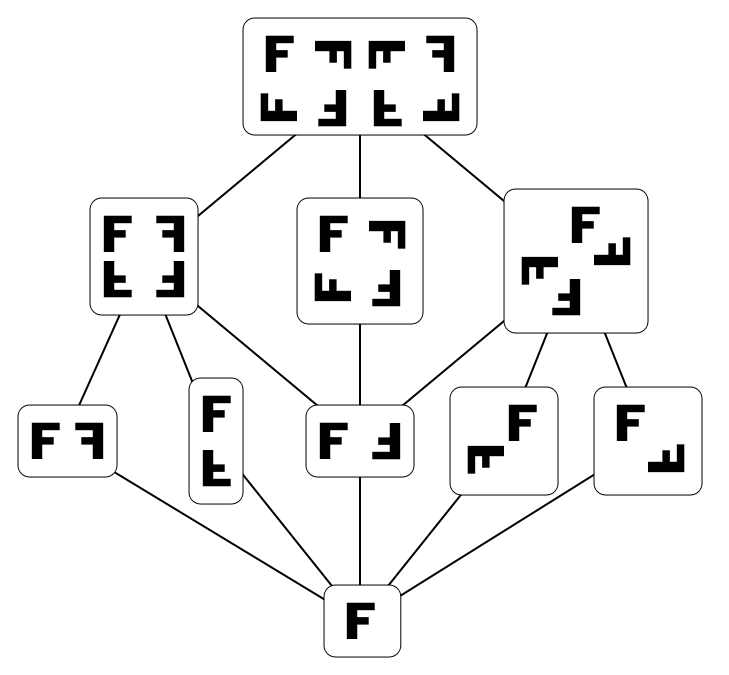
\includegraphics[width=\marginparwidth]{gruppo}
	\caption[Simmetrie del quadrato]{Le simmetrie di un quadrato formano un gruppo di ordine 8. Questo gruppo contiene 1 sottogruppo di ordine 8 (se stesso), 3 sottogruppi di ordine 4, 5 sottogruppi di ordine 2 e 1 sottogruppo di ordine 1 (il sottogruppo \emph{banale}). I sottogruppi sono descritti qui in figura mostrando gli effetti delle singole simmetrie su una figura non simmetrica (la lettera F).}
	\label{fig:gruppo}
}

L’idea di gruppo di sostituzioni è emersa soprattutto in relazione allo studio delle equazioni algebriche, come per esempio l’equazione: $ x^2-2=0 $. In questo caso, si tratta di un’equazione molto semplice da risolvere, ma quando l’equazione è più complessa, in particolare quando è più alto il suo grado, allora il gruppo di sostituzioni permette di risolvere il problema in quella che è ora nota come teoria di Galois.

\section{Il matematico che non aveva tempo}

La mattina del 29 maggio una carrozza viene a prendere Galois. Lo condurrà in una pineta. Non sarà lui il vincitore del duello. A ritrovarlo è un contadino del luogo.

Prima di morire disse al fratello:
”Ho bisogno di tutto il mio coraggio per morire a 20 anni”. 
Il 30 maggio 1832 Évariste Galois muore per traumi subiti allo stomaco da un colpo di arma da fuoco in ospedale. Non aveva nemmeno 20 anni. Viene sepolto in una fossa comune fuori Parigi, dove ancora risiede.

“Mantenete la mia memoria, perché la sorte non mi ha dato abbastanza vita affinché la patria conosca il mio nome”

\medskip

I lavori di Galois rimasero pressoché sconosciuti fino al 1846, quando il matematico francese Joseph Liouville li pubblicò sul suo \emph{Journal de mathématiques pures et appliqueés}, ben 14 anni dopo.

\medskip

Oggi il suo nome è leggenda.

% !TeX spellcheck = it_IT
% !TEX encoding = utf8
% !TEX root = main.tex
\chapter{I 7 ponti di Konigsberg}
Stavo ripassando un po’ di concetti di teoria dei grafi per l’esame, così ho deciso di approfittarne per scrivere la bozza di questo articolo. Il problema dei 7 ponti di Konigsberg è storico e fondamentale per l’evoluzione della matematica discreta. Esso segna l’inizio della teoria dei grafi.

Nella storia della matematica il problema dei ponti di Königsberg è uno dei primi problemi della teoria dei grafi discusso formalmente; esso si può anche considerare uno dei primi problemi concernenti la topologia.

Konigsberg (oggi chiamata Kaliningrad) è una città percorsa dal fiume Pregel e dai suoi affluenti. Presenta due estese isole che sono connesse tra loro e con le due principali aree della città da 7 ponti. Neil 1736 Eulero affrontò il problema dell’esistenza di una passeggiata che permettesse di attraversare tutti i ponti una e una sola volta.

La risposta a tale domanda la scopriremo nei prossimi paragrafi.

ponti di Konigsberg
Descrizione matematica del problema

Essendo tale città composta da due isolotti e da due aree principali, è possibile identificare tali 4 aree con dei punti, dei nodi.

Per schematizzare la situazione, possiamo inoltre trasformare i ponti in archi, linee che congiungono i vari nodi. Non essendovi una direzione di percorrenza dei ponti, possiamo anche evitare di orientare tali archi.

A questo punto ci troviamo davanti ad un grafo (collezione di vertici legati tra loro a due a due da eventuali archi) che schematizza la città nel seguente modo:
ponti di Konigsberg

\begin{figure*}
	\centering
	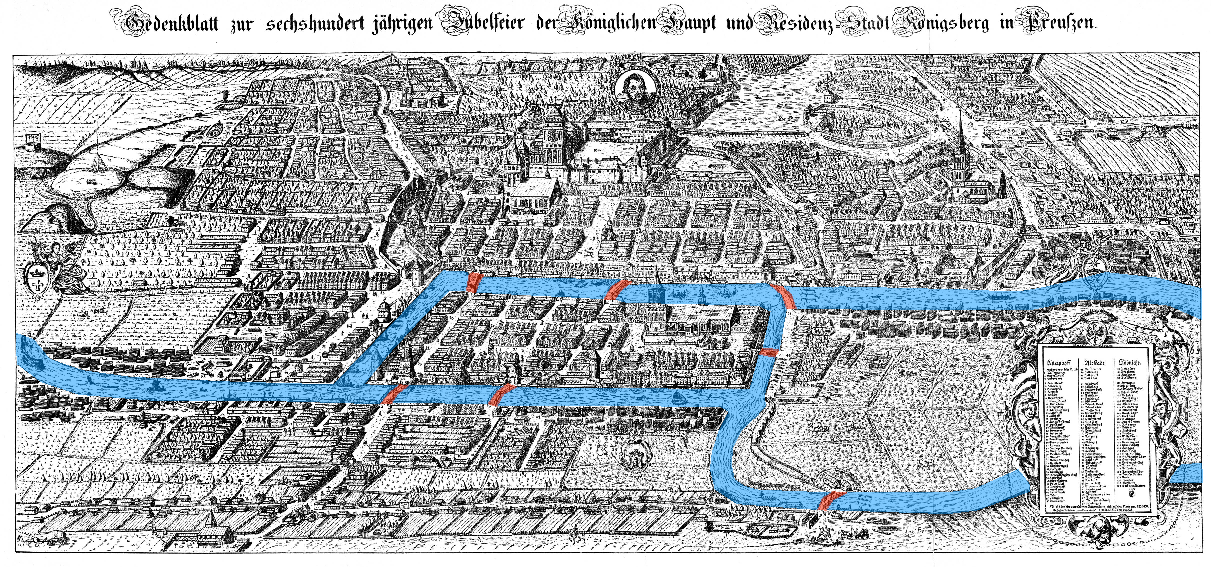
\includegraphics[width=\linewidth]{konigsberg}
\end{figure*}

Dove A,B,C,D sono le quattro zone della città e poi ci sono i vari archi che le connettono, proprio come si vede nell’immagine della città qui sopra.

Ciò che Eulero stava cercando, come molti altri prima di lui,  era un cammino che permettesse di percorrere tutti i ponti esattamente una volta. Provando più e più volte si può vedere come tale risultato non sia raggiungibile.

Ma per fortuna la matematica non è fatta di prove ed errori solamente, ma è fatta di teoremi e risultati generali.

Lui disse e mostrò i due seguenti risultati:

    E’ possibile percorrere tutti gli archi una e una sola volta, concludendo il percorso in un nodo diverso da quello iniziale, se e soltanto se esce un numero dispari di archi soltanto da 2 nodi oppure da nessuno.

Il percorso descritto nelle 3 righe precedenti è detto: Cammino Euleriano

    E’ possibile percorrere tutti gli archi una e una sola volta, concludendo il percorso nel nodo iniziale, se e soltanto se esce un numero pari di archi da tutti i nodi del grafo.

Il percorso qui descritto prende invece il nome di : Ciclo Euleriano.

Chiaramente ciò che stiamo cercando nella città di Konigsberg è un cammino Euleriano. Infatti non abbiamo la pretesa di tornare da dove siamo partiti, ma la necessità di attraversare tutti i ponti una ed una sola volta.

Calcoliamo quindi il grado di tutti e 4 i nodi, dove per grado si intende il numero di archi uscenti dal nodo stesso (in questo caso entranti o uscenti è indifferente dato che non è un grafo orientato).

Il grado di A,B,D è 3, mentre il grado di C è 5. Come si può ben vedere, sono tutti numeri dispari e quindi nessuno tra i due percorsi descritti in precedenza sono presenti nella citta di Konigsberg.

Ecco la risposta alla domanda
Altri due esempi semplici

Devi sapere che l’esistenza di cammini e cicli Euleriani in grafi è esattamente ciò che cercavi da piccolo quando provavi a disegnare una stella o una casetta senza staccare la matita dal foglio!

ponti di Konigsberg

ponti di KoningsbergPoniamoci quindi un paio di domande per descrivere “matematicamente” questi due oggetti che sembrano così semplici. Esiste un solo modo per tracciare tali disegni senza staccare la penna dal foglio? Perchè è possibile disegnarli? Si inizia e finisce il disegno nello stesso punto?

Per rispondere a queste, partiamo dalla casetta. Infatti i due disegni si comportano in modo molto diverso rispetto alle questioni sollevate nelle domande precedenti.

La casetta ha tutti nodi di grado pari, tranne i due nodi alla base. Essi hanno grado dispari: tre. Ecco spigato il motivo per cui sia possibile costruire la casetta senza staccare la penna, infatti tale grafo connesso ammette cammino euleriano, dato che ha esattamente 2 nodi di grado dispari. Ammette però ciclo euleriano? No, per lo stesso motivo, altrimenti dovrebbero essere tutti nodi pari.

Dicendo che esiste un cammino euleriano abbiamo implicitamente detto anche che qualsiasi disegno che ci consenta di tracciare la casetta inizi e finisca in due nodi diversi della casa. Ma resta un’ultima domanda: esiste un solo modo per disegnarla? Beh, in realtà ne esistono due. Infatti il motivo per cui si debbano avere esattamente due nodi dispari per tracciare un cammino euleriano è che l’arco che li rende rispettivamente dispari viene utilizzato per uscire dal nodo iniziale e per entrare nel nodo finale per concludere il disegno.

Prova a pensarci un attimo…se un nodo ha grado pari, ci entro tante volte quante ci esco. Ma nel nodo iniziale io esco una volta in più di quelle che entro, mentre in quello finale entro una volta in più di quelle che esco. Quindi ogni cammino euleriano che posso costruire inizia in un nodo dispari e conclude nell’altro dispari, ecco il perchè della duplicità del cammino euleriano e della possibilità di tracciare la casetta.

Per la stella il discorso è un pelo diverso. Se ci fai caso, infatti, la stella ha tutti i nodi di grado pari. In ogni vertice della stella infatti entrano esattamente due archi. Quindi esiste un ciclo euleriano, ovvero un cammino euleriano che inizia e finisce nello stesso nodo.

Ecco perchè posso tracciare la stella senza staccare la penna dal foglio. Ma ho un solo modo per tracciarla? Beh, in realtà in questo caso possono iniziare da uno qualsiasi dei 5 nodi disponibili. Inoltre posso scegliere il tragitto che più preferisco, infatti il grafo è connesso e tutti i nodi sono di grado pari, quindi comunque scelga ho la certezza di entrare in ogni nodo lo stesso numero di volte che ne uscirò.

Interessante come possa esserci della matematica anche nei giochini che facevi con gli amici alle elementari, vero?

Sulla teoria dei grafi si potrebbe dire ancora davvero molto, ma di sicuro se vedo che piace l’argomento dedicherò a tali tematiche ancora vari articoli. A me piace scoprire nuovi risultati e approfondimenti su questi temi, quindi sarei solo che contento di scriverne ancora

Ti lascio un paio di approfondimenti e riferimenti nel caso ti avessi stimolato almeno un po’ a scoprire il grande mondo dei grafi (o geometria delle posizioni, come Eulero definì questo settore della matematica):

    La matematica dei Social Network: introduzione alla teoria dei grafi 
    Introduction to graph theory
    Graph theory
    Sette ponti di Koningsberg UNIMI: PDF
    Dai ponti di Konigsberg al postino cinese
    I sette ponti di Koningsberg UNITO: PDF

Se vuoi vederti un video ben fatto sull’argomento, ti consiglio questo:

e questo

 

Se invece ti fa piacere rileggerti l’articolo con calma, lo puoi scaricare come PDF cliccando sul bottone qui sotto:
SCARICA IL PDF
Condividi:
\chapter{Il Nobel per la Matematica}
Fisica, chimica, medicina, letteratura, economia e mate... NO! Tra tutte le scienze proprio la matematica, quella che Gauss aveva definito la Regina della scienze e che Galileo aveva definito il Linguaggio dell'Universo, viene esclusa dal florilegio delle declinazioni del famoso premio. Ma perchè? Perchè non esiste il Nobel della Matematica?

\section{Nobel per la matematica}
\marginpar{
	\captionsetup{type=figure}
	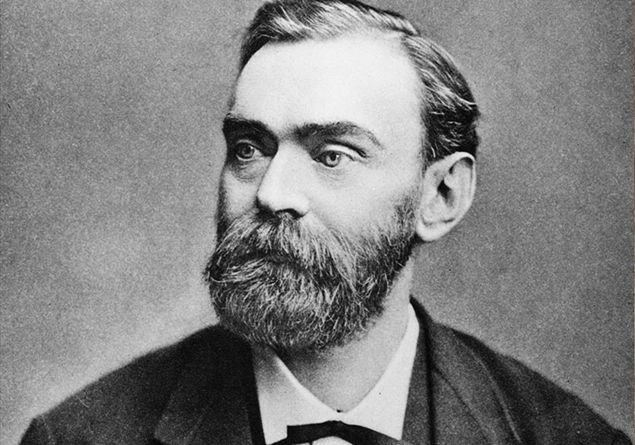
\includegraphics[width=\marginparwidth]{Nobel}
	\caption[Ritratto di Alfred Nobel]{Ritratto di Alfred Nobel}
	\label{fig:AlfredNobel}
}

Come mai non c’è il Nobel per la matematica?

Beh la domanda sorge abbastanza spontanea e anche con un po' di perplessità e amarezza. Facciamo dunque un passo indietro e capiamo dove nasce il famoso premio...

Il premio prende il nome da Alfred Nobel, l’industriale e chimico svedese che ha inventato la dinamite. È stato lui, con le sue ultime volontà, a istituire il prestigioso riconoscimento. Ma perché? La filantropia non sempre si può spiegare, ma nel caso di Nobel forse sì.

La storia, abbastanza veritiera dato che è comprovata da numerose fonti autorevoli, dice che Nobel era negli ultimi anni della sua vita tormentato da avere creato un tale strumento distruttivo... Come se ciò non bastasse, alla morte del fratello nel 1888 la stampa, avendo scambiato il celebre Alfred con il fratello Ludvig, sentenziò a caratteri cubitali "Morto il mercante di morte". Al senso di colpa si aggiungeva quindi anche il danno d’immagine.

Il denaro può dunque migliorare l'opinione che la gente ha di te? Beh a posteriori si direbbe di si! Fu dunque istituito un premio a favore di chi fosse riuscito a apportare «considerevoli benefici all’umanità».

Nobel per la matematica
La leggenda si mischia alla storia

La domanda iniziale rimane comunque ancora aperta... Perchè tra tutte le vie in cui qualcuno potrebbe migliorare la vita dell'Umanità, non ci sarebbe la Matematica?! Leggenda vuole che il signor Nobel l'abbia esclusa per gelosia: sua moglie l'avrebbe tradito con un illustre matematico, lo svedese Gösta Mittag-Leffler.

Beh, purtroppo, sebbene pittoresca e curiosa, questa storia è sostanzialmente falsa! Nobel non è mai stato sposato! Alcuni hanno avanzato ipotesi che i due si odiassero ma, nonostante entrambi fossero di Stoccolma, non hanno avuto molte occasioni per conoscersi perché il primo ha lasciato la Svezia per Parigi quando il secondo era ancora uno studente.

Ma allora perché la matematica è stata tagliata fuori? Non c’è una risposta certa.

Quando il premio è stato creato, però, esisteva già un riconoscimento internazionale per la matematica istituito dal re di Svezia Oscar II: forse Nobel voleva evitare un doppione. O forse, più banalmente, non reputava la matematica capace di apportare «considerevoli benefici all’umanità».
A che premi può dunque ambire un matematico?

Ok, ammettiamolo, oltre alla gloria eterna conferita da un Nobel, a chiunque farebbe gola anche il milioncino che ci arriva correlato (anche se è vero che molti ricercatori devolvono il premio alla ricerca). Tuttavia anche i matematici hanno svariati premi a cui ambire... il più famoso è sicuramente il premio Clay, di cui abbiamo già parlato ampiamente nell'articolo dei 7 problemi da un milione di dollari!.

Oltre a ciò c'è il famoso premio Abel, dato per la prima volta nel 2003 e di cadenza annuale, con "lo scopo di promuovere la matematica, rendendo più prestigiosa questa scienza, specialmente agli occhi delle nuove generazioni". L'ammontare in denaro è all'incira di un milione di dollari anche per questo premio.

Ma nonostante il guadagno economico non sia così grande, il vero Nobel per la Matematica è la Medaglia Fields e viene data ogni 4 anni (giusto per renderla ancora più prestigiosa) e, come se ciò non bastasse, la si può dare solo a ricercatori con meno di 41 anni.

\textit{C'est la vie}, come si dice qui in Francia.
% !TeX encoding = UTF-8
% !TeX spellcheck = it_IT
% !TEX root = main.tex

\chapter{Cos'è un algoritmo? Definizione e qualche esempio}
Cos'è un algoritmo? Eh, domanda non troppo facile ma senz'altro di fondamentale importanza. Ormai siamo nell'era digitale, dove gli algoritmi regano sovrani. Tutti i dispositivi che utilizziamo quotidianamente sono basati su essi, direi quindi che un po' di loro conoscenza non guasta a nessuno ;) .Cos'è un algoritmo?

\section{Introduzione ed esempi pratici}

Per definire questo "oggetto", vediamo di partire da un semplice esempio ;) Sai preparare la pasta giusto? Bene, mentre la prepari segui un algoritmo ben preciso:

\begin{enumerate}
	\item Metti l'acqua nella pentola
	\item Accendi il fuoco e sopra ci metti la pentola
	\item Aspetti 5-10 minuti che l'acqua bolla
	\item Pesi la pasta su una bilancia
	\item Aggiungi il sale all'acqua
	\item Aggiungi la pasta nella pentola
	\item Aspetti 5-10 minuti di cottura
	\item Al termine la scoli e la aggiungi al sugo.
	\item Quindi la servi nel piatto
\end{enumerate}

Chiaramente non fissiamoci troppo sui dettagli della preparazione della pasta, magari tu hai una ricetta super segreta diversa da questa ;) Comunque l'importante è rendersi conto che esistono delle istruzioni che vanno bene in qualsiasi momento per prepararla e funzionano sia che le metta in pratica io che tu. Inoltre il risultato è sempre lo stesso, un bel piattone di pasta 

Vediamo quindi di estrarre le proprietà fondamentali di un algoritmo a partire da questo semplice esempio. Esso è una sequenza di istruzioni/azioni che vanno eseguite in un ordine specifico. Questa sequenza è inoltre finita in tempo, nel senso che sai già che riuscirai a preparare il tuo piatto di pasta in 15-20 minuti. Inoltre questa ricetta non può essere ambigua, interpretabile, ma deve funzionare chiunque sia il "cuoco". Per concludere, le istruzioni devono essere elementari, semplici, non ulteriormente spezzabili in azioni più semplici.

Vediamo quindi un esempio più matematico prima di arrivare a definirli formalmente ;)

\subsection*{Algoritmo di Euclide}

É un algoritmo che si usa per trovare il massimo comun divisore tra due numeri naturali qualsiasi. Se non sai cosa sia il massimo comun divisore (MCD), è semplicemente il numero naturale più grande in grado di dividere esattamente i numeri di partenza. Quindi si ha che esso è uguale ad 1 nel caso essi siano coprimi, ovvero privi di divisori comuni.

Ecco l'algoritmo scritto in linguaggio comune (pseudocodice):

\begin{verbatim}
	Prendi a,b numeri naturali
	Definisci una variabile naturale r
	Finchè b diverso da 0 :
		r = a % b (il resto della divisione tra a e b)
		a = b
		b = r 
	
	Restituisci a
\end{verbatim}

Ora non sto qui troppo a soffermarmi sul perchè questo algoritmo funzioni, magari dai una letta qui ALGORITMO MCD DI EUCLIDE, qualche spunto interessante lo troverai di sicuro ;)

Ciò che importa  per il nostro obiettivo attuale è notare come le operazioni che questo algoritmo comporta sono elementari: divisioni intere e sostituzioni di variabili, niente di più.

Inoltre questo algoritmo fa al più $ b $ iterazioni del ciclo, nel caso in cui essi siano coprimi e quindi termina in tempo finito :) Proprio come avevamo notato prima nell'algoritmo per la pasta.

Chiaramente questo è un algoritmo ancora semplice, in fondo all'articolo ti indicherò alcuni algoritmi grossi e importanti così da farti venire voglia di approfondire l'argomento da solo ;)

\section{Definizione più rigorosa del concetto di \textit{algoritmo}}

\begin{defn}
	Si dice algoritmo una sequenza finita e ordinata di operazioni elementari e non ambigue che permettono di risolvere, in maniera deterministica, un problema in tempo finito, ovvero l'algoritmo ha un termine.
\end{defn}

Se non hai mai sentito parlare di algoritmo in termini un po' più formali, è molto probabile che ti sfugga l'importanza di qualcuna delle richieste che l'algoritmo deve soddisfare per essere definito tale.

Vediamo quindi un paio di esempi che sembrerebbero algoritmi ma non lo sono perchè non rispettano una o più di queste strane proprietà.

Un esempio semplice di non determinismo di una sequenza di istruzioni potrebbe essere introdotta nella procedura di preparazione della pasta. Per esempio si decide che appena si è messa l'acqua a bollire si lancia un dado e a seconda del numero che esce si salterà una delle operazioni che abbiamo elencato successivamente. Non solo questa procedura non è deterministica ma non è nemmeno detto che ci permetta di ottenere il risultato finito :)

Un altro "algoritmo" molto semplice ma che non può essere definito tale in quanto non termina è il seguente:

\begin{verbatim}
	a = 2

Finchè a è pari:

a = 2a

Restituisci a
\end{verbatim}
Chiramente se moltiplichiamo un numero pari per 2, esso rimarrà pari ;) Può sembrare stupido come esempio, ma è sufficientemente chiaro per capire l'importanza di queste proprietà nella buona caratterizzazione di un algoritmo.

Per finire questa carrellata di esempi di non algoritmi, discutiamo un attimo della non ambiguità. Un esempio molto semplice, legato per sempre alla preparazione della pasta, è il seguente:

Nella ricetta invece di dire dopo 10 minuti spegni il fuoco e scola la pasta, supponi di dire di scolarla quando ti sembra cotta.

Il "sembrare cotta" non è chiaramente un parametro oggettivo. Sono d'accordo che nella realtà lo si dice, ma non è un problema dato che noi non siamo macchine ma uomini e donne pensanti, in grado di fare delle scelte in autonomia. Però se si dicesse così ad un computer, o comunque dare queste istruzioni ad una planetaria o un robottino che cucina per te, è ovvio che lui non sarebbe in grado di decidere quando scolare la pasta (a meno di insegnarglielo, ma questo è un discorso più complicato) ;) Ecco il perchè dell'importanza della non ambiguità delle istruzioni.

Proprio perchè queste proprietà devono appartenere ad un qualsiasi algoritmo, essi sono anche rappresentabili mediante un diagramma di flusso. Qui sotto ti allego una immagine tipo e in un altro articolo magari approfondiremo la visione grafica degli algoritmi...merita davvero più spazio che qualche riga stracciata qui.

\begin{figure*}
	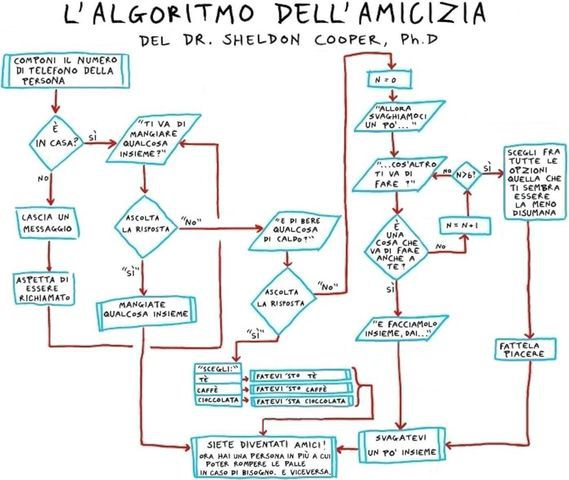
\includegraphics[width=\textwidth]{amicizia}
	\caption{Fonte dell'immagine: Nonciclopedia}
\end{figure*}

Prima di concludere l'articolo, ti lascio un elenco con alcuni algoritmi interessanti a cui ti consiglio di dare un'occhiata. Se c'è interesse, magari ne approfondiremo qualcuno nei prossimi articoli, in caso faccelo sapere mandando un messaggio alla Pagina Facebook, lasciando un commento qui sotto al post o mandando una mail all'indirizzo list@mathone.it :)

\section{Alcuni algoritmi interessanti da approfondire}

Preferisco sviluppare questa sezione in maniera molto schematica, lasciandoti una semplice lista di link che rimandano ad una pagina di approfondimento dedicata al particolare algoritmo, per parlarne sul sito ci sarà tempo in futuro :)

\begin{itemize}
	\item Algoritmo di ricerca di Google
	\item Algoritmi di ordinamento
	\item Algoritmo di Dijkstra (distanza minima)
	\item Algoritmi di raccomandazione
	\item Algoritmi di compressione dati senza perdita
\end{itemize}

Ce ne sarebbero molti altri ma per ora direi che è una lista anche troppo lunga, se vuoi guardare qualcos'altro su questo sito, ecco alcuni articoli legati a queste tematiche che avevamo scritto in passato:

Algoritmo calcolo radice quadrata
Algoritmo moltiplicazione egizia
Alla scoperta di algoritmi antichi e curiosi
% !TeX encoding = UTF-8
% !TeX spellcheck = it_IT
% !TEX root = main.tex
\chapter{Turbolenza: introduzione a questo strano e complesso fenomeno}
Turbolenza, un fenomeno che siamo abituati ad osservare quotidianamente in natura ma che la matematica difficilmente domina al momento. E' meraviglioso come possa essere complicato descrivere con equazioni situazioni che siamo soliti dare per scontate. Chi direbbe mai che non siamo in grado di comprendere pienamente il perchè l'acqua che esce dal rubinetto si muove in quel modo, oppure perchè l'aria si distribuisca in modo particolare attorno al profilo alare di un aereo... ;)

In questo articolo, faremo un breve viaggio alla scoperta del concetto di turbolenza, analizzando i risultati ai quali la ricerca è riuscita ad arrivare al momento e le domande ancora aperte. Non voglio che diventi un articolo noioso, ma essendo uno degli articoli più applicativi che ho scritto fino ad ora ho intenzione di presentarti molti esempi e immagini :) Inoltre ti avviso già che è un articolo lungo, però per introdurre la turbolenza con un minimo di completezza e matematica è stato necessario...

La turbolenza è attualmente uno dei più grandi problemi fisici ancora aperti ed irrisolti. E' strettamente legata alla complessità delle equazioni che regolano la dinamica dei fluidi (di Navier-Stokes), uno dei problemi del millennio. Se non sai di cosa sto parlando, dai una letta all'articolo che aveva scritto Erik sui Problemi del millennio al Capitolo \ref{ch:millenium_problems}.

Magari ci concentreremo un'altra volta su queste equazioni. Per ora mi interessa evidenziare solamente il fatto che sono \textit{equazioni differenziali alle derivate parziali} (PDE) fortemente \emph{non lineari}. Sono un sistema misto di equazioni iperboliche e paraboliche e la caoticità delle loro soluzioni è la motivazione alla base del comportamento turbolento delle correnti.

Le precedenti 4-5 righe, sono dedicate a chi la matematica la mastica abbastanza bene. 
\footnote{Se hai capito poco o niente non preoccuparti, non è questo il centro dell'articolo che stai leggendo ;)}
Alcune definizioni

Per parlare di argomenti così complessi è chiaramente necessaria una terminologia specifica. Cercando di non appesantire troppo la lettura, ho quindi deciso di dedicare un piccolo paragrafo all'introduzione di alcuni nomi e concetti che ci saranno poi utili.

\begin{defn}[Fluido]
	Una sostanza in grado di reagire a delle "forze" (non è del tutto corretto, in realtà si deve parlare di sforzi ma se non sai cosa siano è lo stesso, basta che passi l'idea) perpendicolari alla superficie da essa individuata e di deformarsi indefinitamente se sottoposta a forze tangenziali esterne.
\end{defn}

\begin{defn}[Densità]
	E' una caratteristica del fluido, essa è una funzione continua dello spazio e del tempo (sotto le opportune ipotesi che non approfondiremo) che rappresenta il rapporto tra la quantità di massa di fluido contenuta in un volume infinitesimo e il volume stesso:
	\[\rho=\lim_{\Delta V\to 0}\frac{M}{\Delta V} \]
\end{defn}
 
\begin{defn}[Viscosità]
	Si dice viscosità la resistenza che gli strati di fluido pongono allo scorrere l'uno sull'altro, intuitivamente è legata allo scambio di quantità di moto tra i vari elementi di fluido.
\end{defn}

\begin{defn}[Corrente]
	Un regime di moto associato ad un particolare fluido, completamente descritto dalla terna pressione, densità e campo di velocità. E' importante specificare che le proprietà che sono associabili alle correnti valgono per ogni fluido che è caratterizzato da quel regime di moto particolare. In seguito parleremo infatti di corrente turbolenta e non di fluido turbolento.
\end{defn}
 
\begin{defn}[Grandezza caratteristica]
	In fisica spesso si cerca di lavorare con numeri e quantità a-dimensionali, per astrarre il più possibile l'analisi (e per motivi strettamente numerici). Per ricondurci a delle equazioni a-dimensionali si ricorre alla divisione delle funzioni in gioco per delle grandezze caratteristiche del moto o della geometria che si sta analizzando. Per esempio se stiamo analizzando la corrente in un fiume, possiamo identificare come lunghezza caratteristica l'ampiezza media del fiume. Oppure se dobbiamo lavorare con delle velocità, possiamo a-dimensionalizzarle dividendole per la velocità media della corrente (che può essere trattata come una velocità caratteristica).
\end{defn} 

Una volta introdotti questi concetti fondamentali, addentriamoci nel vivo della turbolenza partendo dall'esperimento classico condotto da Reynolds per evidenziare la transizione tra un regime di corrente laminare (ordinato) e turbolento (caotico).

\section{L'esperimento di Reynolds}

Quest'esperienza ha l'obiettivo di mostrare come, al variare delle condizioni di una corrente, vari anche il comportamento di un sottile "filo" di colorante introdotto nel condotto che ospita il fluido in moto. Nel video qui sotto puoi vedere come si svolge l'esperimento ;)


Senza analizzarlo troppo, si vede (ed è anche spiegato nel video) che a velocità della corrente sufficientemente basse, il filamento di colorante introdotto nel condotto si muove con regolarità ed ordine in un moto rettilineo. Appena la velocità della corrente cresce, il moto si trasforma in moto caotico, disordinato, variabile ed oscillante nel tempo. Chi l'avrebbe mai detto che un semplice aumento di velocità potesse causare un casino del genere?! ;)

Detto ciò, questo comportamento è esattamente ciò che puoi osservare quando apri il rubinetto dell'acqua. Se ne fai uscire poca alla volta, da esso uscirà un sottile filamento lineare d'acqua, se aumenti la pressione del rubinetto diventerà un getto molto più irregolare e oscillante nella forma.

\section{Turbolenza}

Per me è stato molto strano scoprire di questa diverso comportamento in funzione della velocità della corrente, infatti sono cose a cui purtroppo siamo abituati e di cui non ci poniamo spesso domande.

Ma quindi che caratteristiche ha questo nuovo tipo di corrente che sembra molto più piena e strana? Nel prossimo paragrafo citerò alcune tra le principali proprietà del moto turbolento, evidenziandone alcuni esempi evidenti nella realtà. Spero ti piaccia come approccio al fenomeno ;)
Alcune proprietà della turbolenza

Il moto turbolento della corrente è caratterizzato da:

Tridimensionalità: A differenza del moto laminare che si verifica nel caso del rubinetto che fa uscire un filino d'acqua, non è possibile descrivere il moto che si presenta aumentando la pressione del rubinetto come una corrente parallela. E' evidente che vanno coinvolte 3 dimensioni per descrivere il caos generato dalle linee di corrente dell'acqua e dalle molecole che si urtano molto frequentemente creando delle traiettorie irregolari e quasi imprevedibili.

Vorticità: Nelle equazioni che regolano la vorticità (che è il rotore della velocità) dopo una breve analisi si può ricavare che nel caso di corrente tridimensionale si ha una vorticità che varia lungo le linee di corrente, autoalimentandosi e ripartendosi lungo le varie direzioni a causa delle variazioni di velocità della corrente stessa. La vorticità si dimostra visivamente come la rotazione degli elementi di fluido (insiemi di molecole, o anche individuabili come blocchetti di fludo) su se stessi, ed evidentemete questo aspetto si verifica nell'esperimento visto in precedenza con il colorante. Infatti il filamento lineare ed ordinato che si vede all'inizio poi va a rimescolarsi, a riempire il condotto e a ruotare su se stesso.

Un altro esempio in cui la presenza della vorticità è molto chiara, sono le correnti dei fiumi che devono passare sotto un ponte. Quando le linee di corrente incontrano un palo di sostegno del ponte, si separano in modo caotico, e le porzioni d'acqua iniziano a ruotare su se stesse, creando una situazione molto confusionaria e burrascosa.

La turbolenza è una proprietà multiscala: Un forte ruolo nella ricerca sulla turbolenza e la sua molteplicità di scale è dovuto a Kolmogorov, grande matematico a cui vengono dedicate anche le cosiddette scale di Kolmogorov, ovvero i fenomeni turbolenti sulle microscale. Ma cosa si intende per molteplicità di scale?

Semplicemente la turbolenza non si esplicita allo stesso modo se valutata su spazi molto piccoli (lunghezze caratteristiche ridotte) o su macroscale quali potrebbero essere le analisi fatte sulle lunghezze caratteristiche tipiche del fiume stesso. In particolare, si può notare una cascata energetica a carico della viscosità (che può essere vista come un insieme di forze interne che portano a dissipare energia fino a raggiungere la stabilità) che trasforma i vortici delle macroscale (molto instabili perchè di grandi dimensioni), nei vortici di dimensioni molto ridotte più stabili. A questo punto l'energia rimasta dopo la dissipazione nei vortici stabili, si disperde in calore.

Quindi i vortici delle correnti turbolente non sono solo quelli che vediamo ma c'è molto di più! Questo è uno dei motivi principali per cui l'analisi del regime turbolento delle correnti è molto complicato. Esso infatti non può essere trattato nei rispetti della sua natura seguendo un approccio completamente statistico, basato su medie nel tempo, altrimenti si supporrebbe che ad ogni scala di ingrandimento il fenomeno si esplicita allo stesso modo.

Turbolenza

Non abbiamo tempo e modo di approfondire un approccio statistico alla turbolenza mediante le equazioni mediate di Reynolds (RANS), seppur molto interessante e utilizzato a livello ingegneristico. Tuttavia ti basti sapere che trascura molti aspetti della fisica del fenomeno, però è funzionale per valutare le dinamiche turbolente in quanto permette di ottenere risultati significativi in tempi ragionevoli (a differenza della risoluzione numerica diretta delle equazioni della turbolenza che richiederebbero tempi esorbitanti per lavorare efficacemente).

Apparente casualità: Come ogni fenomeno caotico che si rispetti, non stiamo parlando di un fenomeno stocastico e completamente imprevedibile, ma la turbolenza soffre di una forte sensitività ai dati iniziali. Cosa vuol dire? Beh, semplicemente che se noi proviamo a riprodurre l'evoluzione della corrente turbolenta due volte consecutive con condizioni molto simili tra loro, potremmo avere sviluppi completamente diversi. L'unico modo che abbiamo per essere certi di due sviluppi coincidenti sarebbe rimettere al loro posto tutte le molecole dell'universo nel momento della sua origine ;)

Un esempio molto semplice e visivo di questa sensitività ai dati iniziali tipico delle dinamiche caotiche è il pendolo doppio, la cui lieve variazione del punto di partenza del pendolo causa evoluzioni completamente diverse, come puoi vedere dal video qui sotto:



Potrei elencare altre proprietà, come la dissipazione energetica o l'instazionarietà, ma siccome immagino che ormai ti stai stufando perchè l'articolo è lungo, preferisco passare a riaccendere un po' gli animi proponendoti alcuni esempi, citando il problema da un milione di dollari ad essa legato e dicendo il perchè sia fondamentale il progresso della ricerca matematica in questo campo :)
Un milione di dollari e perchè provarci

Come già detto nelle righe precedenti, accanto alla comprensione della turbolenza, si hanno dei problemi matematici molto grossi, dovuti alla valutazione dell'esistenza o meno di soluzioni delle equazioni di Navier-Stokes per particolari flussi e particolari ipotesi.

Ecco quindi citato testualmente il problema la cui risoluzione porterebbbe a farti guadagnare un milione di dollari ;)

Turbolenza

Ovvero:

Data una condizione iniziale v0 = v(x,0), campo vettoriale nello spazio euclideo, esiste una funzione vettoriale per la velocità v(x,t) e una funzione di pressione p(x,t) che soddisfa le equazioni di Navier-Stokes? Esiste una soluzione se v0 è liscia?

A parte questo spunto e stimolo, mi fa piacere condividere alcuni dei motivi per cui è importante spingere la ricerca in questi campi.

Una maggiore comprensione del fenomeno della turbolenza avrebbe notevoli ricadute tecnologiche ed economiche. Si pensi, ad esempio, al risparmio che si avrebbe se si potesse mantenere laminare (ordinata e regolare) la corrente attorno ad un aereo che vola per dodici ore considerato che la metà del peso al decollo è dato dal carburante. Infatti la transizione che avviene ad alte velocità da moto laminare a turbolento causa una resistenza d'attrito molto più grande dell'area al "fluire" dell'aereo, richiedendo così maggior carburante per gestire l'intero volo.

Turbolenza

Tra i numerosi settori tecnologici in cui compare la turbolenza ricordiamo i processi di combustione, i condotti per il trasporto di gas/petrolio, le scie dietro ai mezzi di trasporto, il comportamento del sangue in arterie/vene (emodinamica), lo studio di aneurismi celebrali, la diffusione di spray ed aerosol.

Insomma, i campi che richiedono un avanzamento degli studi sulla turbolenza sono molti, ecco perchè ritenevo utile provare a scrivere questo articolo, sapendo però che è un rischio dato che non è un argomento semplice e facile da descrivere con poca matematica (ho però cercato di usarla poco, se non niente per questo primo articolo).
Alcuni esempi visivi

Questa sezione ho deciso di svilupparla usando poche parole scritte e proponendoti molti video che secondo me rendono molto di più, soprattutto per farti un'idea e contestualizzare tutto ciò che hai letto fino ad ora :)

Flusso laminare e flusso turboleento in un fiume

Evoluzione strato limite turbolento attorno a lamina piana

Riferimenti per approfondimenti

Come mi è stato consigliato da alcuni di voi, d'ora in poi inizierò ad aggiungere in coda agli articoli alcune risorse per approfondire ciò che si è solamente introdotto nelle righe precedenti. Potrebbero essere libri di testo, libri divulgativi, pdf , video o articoli, dipenderà dal tema e dalle risorse che considero più valide.

Qui di seguito trovi alcuni articoli che trattano l'importanza del problema della turbolenza da un punto di vista fisico e matematico. I primi due sono anche molto rilevanti, a parer mio, perchè il primo spiega il perchè la turbolenza sia ancora un problema matematico aperto e il secondo ne fornisce una comprensione fisica più completa.

Why global regularity for Navier-Stokes is hard
On the nature of turbolence
Un testo sulla dinamica dei fluidi : Fluid Dynamics

Spero di non averti annoiato troppo, ti ringrazio se sei arrivato a leggere fin qui e spero di sentire qualche tuo parere riguardo questa tematica e l'articolo ;)
% !TeX encoding = UTF-8
% !TeX spellcheck = it_IT
% !TEX root = main.tex
\chapter{Problemi del Millennio}
\label{ch:millenium_problems}
% !TeX spellcheck = it_IT
% !TEX encoding = utf8
% !TEX root = main.tex

\chapter{Cédric Villani: il teorema vivente}
Matematico francese, 43 anni, attivo nel campo delle equazioni differenziali e della fisica matematica, conosciuto per il suo look fatto di cravatte da dandy, panciotti con orologio nel taschino e una spilla a forma di ragno sul bavero della giacca. Ma chi é Cédric Villani?! Come mai tutti ne parlano?
\section{Biografia}
\marginpar{
	\captionsetup{type=figure}
	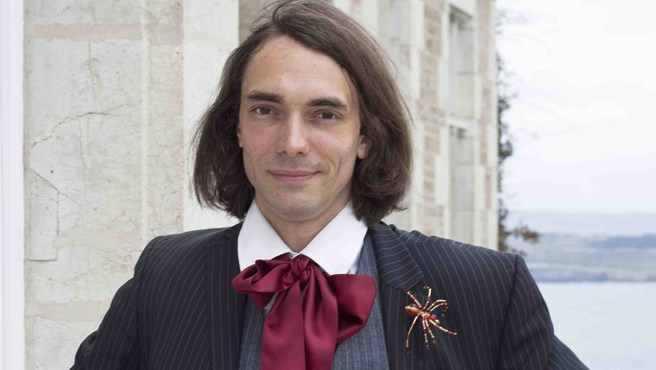
\includegraphics[width=\marginparwidth]{villani.jpg}
	\caption{Cédric Villani}
	\label{fig:villani}
}

Cèdric Villani compie i suoi studi all’\emph{École Normale Superiore} a Parigi (la sorella maggiore della \emph{Scuola Normale} di Pisa, per intenderci, nonchè uno degli istituti più importanti dell’intera Europa) dal 1992 al 1996, dove diventa anche \emph{assistant professor}. Nel 2000 si trasferisce a Lione, dove ottiene la cattedra e lavora tuttora, mentre dal 2009 è anche direttore dell’isituto Poincaré.
Sempre nel 2009 riceve la Medaglia Fermat mentre nel 2010 riceve la Medaglia Fields. Ha solo 37 anni.

Nel 2012 esce il suo celebre libro \emph{\textbf{Théorème vivant}} (il \emph{Teorema vivente}, edito da Rizzoli) nel quale spiega il suo lavoro e cosa vuol dire fare ricerca nel ramo della matematica. Nel 2016 è protagonista del TED talk di Vancouver mentre dal 2016 è un parlamentare della legislazione Macron.

\section{Vita privata e celebrità}
Cédric Villani è considerato un personaggio curioso per il suo aspetto e le sue passioni (divora fumetti manga giapponesi), dotato di un intuito fuori dal comune. Un genio della matematica, un vero ninja, in grado però di spiegare anche i temi più complessi con parole semplici e al grande pubblico. In molti lo hanno conosciuto con la pubblicazione del già citato saggio «Il Teorema vivente. La mia più grande avventura matematica».

Ma cosa fa dunque Cédric Villani? Ebbene i suoi studi riguardano la teoria delle equazioni differenziali alle derivate parziali coinvolte nella meccanica statistica; in particolare sull’equazione di Boltzmann, sulla quale ha vinto la celebre Medaglia. Ha lavorato inoltre sulla teoria del trasporto ottimale e sulle sue applicazioni in geometria differenziale. So che alcuni di voi potrebbero essersi persi, però il tempo di un caffè non è sufficiente per dilungarsi su cosa vertano questi argomenti. Per conoscenza però vi dico solo che sono alcuni degli argomenti più “caldi” della fisica matematica moderna.
\section{Il sogno della «città della scienza»}

A qualcuno leggendo le prossime righe potrebbe tornare in mente Platone e la sua idea della società perfetta guidata dai filosofi… ma vediamo perchè

Nelle ultime elezioni legislative francesi è stato candidato per il dipartimento francese della regione dell’Ile-de-France (Francia sud, per capirci, dove ci sono Lione, Grenoble e Saclay). Proprio là dove si trova la città di Saclay, considerata la Silicon Valley alla francese, e dove Villani avrebbe il desiderio di creare una cittadella della scienza e della tecnologia. Questo progetto è da molti considerato quasi utopico, ma se ci crede una Medaglia Fields, merita di farci un pensierino…

Spero con queste poche righe di avere suscitato in voi l’interesse per questa eclettica persona dagli interessi più svariati. Per approfindimento ti consiglio l'intervista sul sito di Madmaths citata nella Bibliografia \cite{url:maddmath_villani}! Attualmente in Francia è considerato come una celebrità e di sicuro se ne sentirà ancora parlare di lui.

\bibliography{bibliography}

\end{document}
